\documentclass[12pt,a4paper]{article}
\usepackage[utf8]{vietnam}
\usepackage{amsmath,amssymb}
\usepackage{tikz}
\usetikzlibrary{calc,angles,quotes,arrows.meta,positioning}
\usepackage[top=1.5cm, bottom=1.5cm, left=1.8cm, right=1.8cm]{geometry}

\begin{document}
\section*{Câu 4. Tam giác ABC có phân giác AD và BE}
\begin{center}
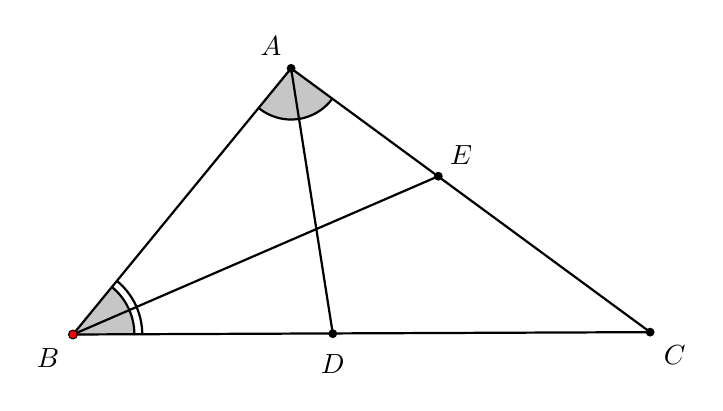
\begin{tikzpicture}[scale=1, line cap=round, line join=round, >=Stealth]
  % Toạ độ điểm (1 đơn vị = 1 cm)
  \coordinate (A) at (2.77,3.38);
  \coordinate (B) at (0,0);
  \coordinate (C) at (7.33,0.03);
  \coordinate (D) at (3.30,0.01);
  \coordinate (E) at (4.64,2.01);

  % Góc A: tô xám và vẽ cung (bán kính 0.65)
  \fill[gray!45] (A) -- ++(230.67:0.65) arc[start angle=230.67, end angle=323.7, radius=0.65] -- cycle;

  % Góc B: tô xám (bán kính 0.78)
  \fill[gray!45] (B) -- (0.78,0.003) arc[start angle=0.2, end angle=50.67, radius=0.78] -- cycle;

  % Các cạnh tam giác
  \draw[thick] (A) -- (B) -- (C) -- cycle;

  % Hai đường phân giác AD, BE
  \draw[thick] (A) -- (D);
  \draw[thick] (B) -- (E);

  % Cung góc tại A (1 cung)
  \draw[thick] ($(A)+(230.67:0.65)$) arc[start angle=230.67, end angle=323.7, radius=0.65];

  % Cung góc tại B (2 cung)
  \draw[thick] (0.78,0.003) arc[start angle=0.2, end angle=50.67, radius=0.78];
  \draw[thick] (0.88,0.003) arc[start angle=0.2, end angle=50.67, radius=0.88];

  % Các điểm
  \foreach \p in {A,C,D,E}{
    \fill (\p) circle (1.6pt);
  }
  \filldraw[fill=red, draw=black, line width=0.4pt] (B) circle (1.6pt);

  % Nhãn đỉnh
  \node[above left=1pt and 0pt] at (A) {$A$};
  \node[below left=2pt]         at (B) {$B$};
  \node[below right=2pt]        at (C) {$C$};
  \node[below=4pt]              at (D) {$D$};
  \node[above right=1pt]        at (E) {$E$};
\end{tikzpicture}
\end{center}

\vspace{0.5cm}
\section*{Câu 5. Hai đường thẳng song song a // b}
\begin{center}
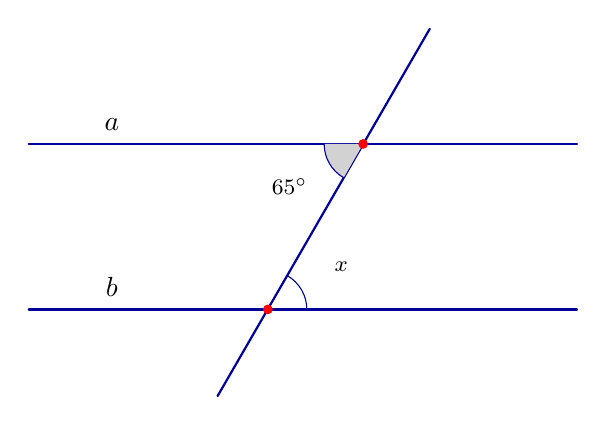
\begin{tikzpicture}[scale=1.1, line cap=round, line join=round]
  % Toa do chuan (don vi 1cm ~ 100px anh goc), cat tuyen nghieng 60 do
  \coordinate (B) at (0,0);          % giao diem cat tuyen voi b
  \coordinate (A) at (1.10,1.91);    % giao diem cat tuyen voi a

  % Hai duong thang song song a, b
  \draw[thick, blue!60!black] (-2.76,1.91) -- (3.57,1.91);
  \draw[thick, blue!60!black] (-2.76,0)    -- (3.57,0);

  % Cat tuyen
  \draw[thick, blue!60!black] (-0.58,-1.00) -- (1.87,3.24);

  % Goc 65 do tai A (duoi a, ben trai cat tuyen): tu 180 do den 240 do
  \fill[gray!35] (A) -- ++(180:0.45) arc[start angle=180, end angle=240, radius=0.45] -- cycle;
  \draw[blue!60!black, thin] (A) ++(180:0.45) arc[start angle=180, end angle=240, radius=0.45];
  \node[font=\footnotesize] at ($(A)+(210:0.98)$) {$65^\circ$};

  % Goc x tai B (tren b, ben phai cat tuyen): tu 0 do den 60 do
  % (Neu can goc trong cung phia ben trai: doi sang arc 60 -> 180, nhan tai goc 120 do)
  \draw[blue!60!black, thin] (B) ++(0:0.45) arc[start angle=0, end angle=60, radius=0.45];
  \node[font=\footnotesize] at ($(B)+(30:0.98)$) {$x$};

  % Diem giao
  \fill[red] (A) circle (1.6pt);
  \fill[red] (B) circle (1.6pt);

  % Ten duong thang
  \node[above] at (-1.80,1.95) {$a$};
  \node[above] at (-1.80,0.04) {$b$};
\end{tikzpicture}
\end{center}

\vspace{0.5cm}
\section*{Câu 7. Trục số điểm A}
\begin{center}
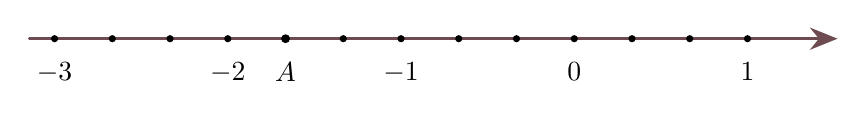
\begin{tikzpicture}[x=2.2cm, y=1cm, scale=1, line cap=round, line join=round, >=Stealth]
  % Màu nét trục số (nâu xám như trong ảnh)
  \definecolor{axiscol}{RGB}{110,75,80}

  % Trục số có mũi tên sang phải
  \draw[axiscol, line width=1.2pt, -{Stealth[length=3.5mm, width=2.8mm]}] (-3.145,0) -- (1.52,0);

  % Các chấm chia: mỗi đoạn đơn vị chia 3 phần bằng nhau (từ -3 đến 1)
  \foreach \i in {0,1,...,12} {
    \fill ({-3+\i/3},0) circle (1.3pt);
  }

  % Nhãn các số nguyên (đặt phía dưới trục)
  \node[below=5pt] at (-3,0) {$-3$};
  \node[below=5pt] at (-2,0) {$-2$};
  \node[below=5pt] at (-1,0) {$-1$};
  \node[below=5pt] at (0,0)  {$0$};
  \node[below=5pt] at (1,0)  {$1$};

  % Điểm A tại -1 2/3 = -5/3 (chấm đen và nhãn A)
  \fill (-5/3,0) circle (1.6pt);
  \node[below=5pt] at (-5/3,0) {$A$};
\end{tikzpicture}
\end{center}

\vspace{0.5cm}
\section*{Câu 10. Bốn hình lăng trụ/hình khối}
\begin{center}
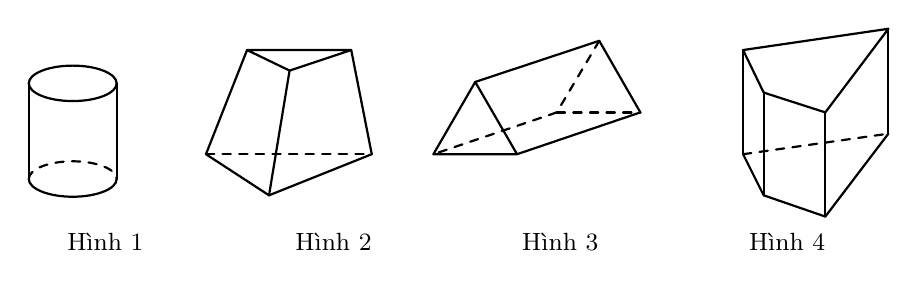
\begin{tikzpicture}[scale=0.9, line cap=round, line join=round, thick]

  % ===== Hình 1: hình trụ =====
  \draw (0.04,1.67) -- (0.04,0.32);
  \draw (1.28,1.67) -- (1.28,0.32);
  \draw (0.66,1.67) ellipse (0.62 and 0.25);
  \draw (0.04,0.32) arc (180:360:0.62 and 0.25);
  \draw[dashed] (0.04,0.32) arc (180:0:0.62 and 0.25);
  \node at (1.12,-0.57) {\small Hình 1};

  % ===== Hình 2: hình chóp cụt tam giác =====
  \coordinate (A1) at (3.12,2.14);
  \coordinate (B1) at (4.59,2.14);
  \coordinate (C1) at (3.72,1.85);
  \coordinate (A2) at (2.54,0.67);
  \coordinate (B2) at (4.88,0.67);
  \coordinate (C2) at (3.43,0.09);

  \draw (A1) -- (B1) -- (C1) -- cycle;
  \draw (A1) -- (A2);
  \draw (B1) -- (B2);
  \draw (C1) -- (C2);
  \draw (A2) -- (C2) -- (B2);
  \draw[dashed] (A2) -- (B2);
  \node at (4.34,-0.57) {\small Hình 2};

  % ===== Hình 3: lăng trụ đứng tam giác nằm ngang =====
  \coordinate (P1) at (5.75,0.67);
  \coordinate (P2) at (6.93,0.67);
  \coordinate (P3) at (6.34,1.69);
  \coordinate (Q1) at (7.49,1.26);
  \coordinate (Q2) at (8.67,1.26);
  \coordinate (Q3) at (8.09,2.27);

  \draw (P1) -- (P2) -- (P3) -- cycle;
  \draw (P3) -- (Q3);
  \draw (Q3) -- (Q2);
  \draw (P2) -- (Q2);
  \draw[dashed] (Q3) -- (Q1);
  \draw[dashed] (Q1) -- (Q2);
  \draw[dashed] (Q1) -- (P1);
  \node at (7.54,-0.57) {\small Hình 3};

  % ===== Hình 4: lăng trụ đứng đặt thẳng đứng =====
  \coordinate (U1) at (10.12,2.14);
  \coordinate (U2) at (10.41,1.54);
  \coordinate (U3) at (11.28,1.26);
  \coordinate (U4) at (12.17,2.44);
  \coordinate (D1) at (10.12,0.67);
  \coordinate (D2) at (10.41,0.09);
  \coordinate (D3) at (11.28,-0.21);
  \coordinate (D4) at (12.17,0.96);

  \draw (U1) -- (U2) -- (U3) -- (U4) -- cycle;
  \draw (U1) -- (D1);
  \draw (U2) -- (D2);
  \draw (U3) -- (D3);
  \draw (U4) -- (D4);
  \draw (D1) -- (D2) -- (D3) -- (D4);
  \draw[dashed] (D1) -- (D4);
  \node at (10.74,-0.57) {\small Hình 4};

\end{tikzpicture}
\end{center}

\vspace{0.5cm}
\section*{Câu 11. Bốn hình khối lăng trụ/hình hộp}
\begin{center}
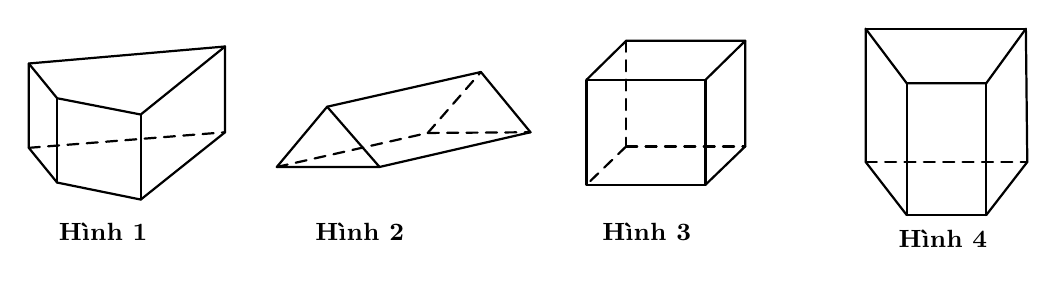
\begin{tikzpicture}[scale=0.9, line cap=round, line join=round, x=1cm, y=1cm]
  \tikzset{
    vis/.style={thick},
    hid/.style={thick, dash pattern=on 4pt off 3pt}
  }

  % ===== Hình 1 =====
  \coordinate (A1) at (0.12,2.47);
  \coordinate (B1) at (0.52,1.98);
  \coordinate (C1) at (1.70,1.75);
  \coordinate (D1) at (2.89,2.71);
  \coordinate (E1) at (0.12,1.28);
  \coordinate (F1) at (0.52,0.79);
  \coordinate (G1) at (1.70,0.55);
  \coordinate (H1) at (2.89,1.50);

  \draw[vis] (A1)--(D1)--(H1)--(G1)--(F1)--(E1)--cycle;
  \draw[vis] (A1)--(B1)--(C1)--(D1);
  \draw[vis] (B1)--(F1);
  \draw[vis] (C1)--(G1);
  \draw[hid] (E1)--(H1);
  \node at (1.17,0.10) {\small\bfseries Hình 1};

  % ===== Hình 2 =====
  \coordinate (A2) at (3.62,1.01);
  \coordinate (B2) at (4.33,1.86);
  \coordinate (C2) at (5.07,1.01);
  \coordinate (D2) at (6.50,2.35);
  \coordinate (E2) at (7.20,1.50);
  \coordinate (F2) at (5.75,1.49);

  \draw[vis] (A2)--(B2)--(C2)--cycle;
  \draw[vis] (B2)--(D2)--(E2)--(C2);
  \draw[hid] (A2)--(F2);
  \draw[hid] (F2)--(D2);
  \draw[hid] (F2)--(E2);
  \node at (4.79,0.10) {\small\bfseries Hình 2};

  % ===== Hình 3 =====
  \coordinate (A3) at (7.99,2.24);
  \coordinate (B3) at (9.67,2.24);
  \coordinate (C3) at (9.67,0.76);
  \coordinate (D3) at (7.99,0.76);
  \coordinate (A3') at (8.55,2.79);
  \coordinate (B3') at (10.23,2.79);
  \coordinate (C3') at (10.23,1.30);
  \coordinate (D3') at (8.55,1.30);

  \draw[vis] (A3)--(B3)--(C3)--(D3)--cycle;
  \draw[vis] (A3)--(A3')--(B3')--(B3);
  \draw[vis] (B3')--(C3')--(C3);
  \draw[hid] (A3')--(D3');
  \draw[hid] (D3')--(C3');
  \draw[hid] (D3')--(D3);
  \node at (8.84,0.10) {\small\bfseries Hình 3};

  % ===== Hình 4 =====
  \coordinate (A4) at (11.93,2.96);
  \coordinate (B4) at (14.19,2.96);
  \coordinate (C4) at (12.51,2.19);
  \coordinate (D4) at (13.63,2.19);
  \coordinate (E4) at (12.51,0.33);
  \coordinate (F4) at (13.63,0.33);
  \coordinate (G4) at (11.93,1.08);
  \coordinate (H4) at (14.21,1.08);

  \draw[vis] (A4)--(B4);
  \draw[vis] (A4)--(C4)--(D4)--(B4);
  \draw[vis] (C4)--(E4)--(F4)--(D4);
  \draw[vis] (A4)--(G4)--(E4);
  \draw[vis] (B4)--(H4)--(F4);
  \draw[hid] (G4)--(H4);
  \node at (13.02,0.00) {\small\bfseries Hình 4};
\end{tikzpicture}
\end{center}

\vspace{0.5cm}
\section*{Phần II Câu 2. Vuông góc CD và các góc tại B, A}
\begin{center}
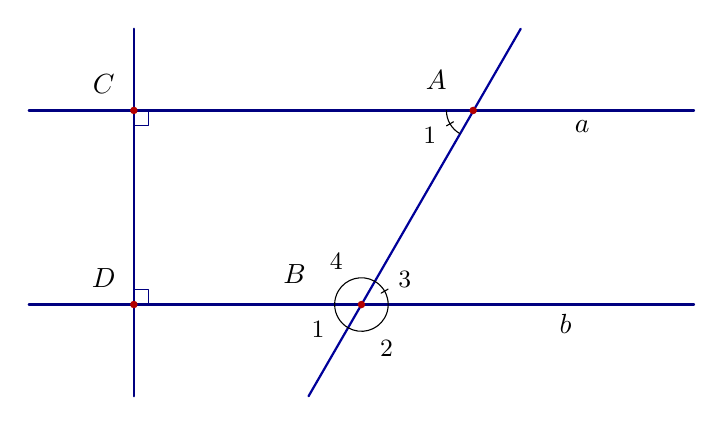
\begin{tikzpicture}[scale=0.85, line cap=round, line join=round, >=stealth]
  % Điểm chuẩn (đơn vị: cm, D là gốc tọa độ)
  \coordinate (D) at (0,0);
  \coordinate (C) at (0,2.9);
  \coordinate (B) at (3.4,0);
  \coordinate (A) at (5.07,2.9);

  % Đường thẳng a, b và CD
  \draw[thick, blue!50!black] (-1.57,2.9) -- (8.37,2.9);
  \draw[thick, blue!50!black] (-1.57,0)   -- (8.37,0);
  \draw[thick, blue!50!black] (0,-1.37)   -- (0,4.12);

  % Cát tuyến qua B và A (nghiêng 60° so với b)
  \draw[thick, blue!60!black] (2.61,-1.37) -- (5.78,4.12);

  % Ký hiệu góc vuông tại C và D
  \draw[blue!50!black] (0,0.22) -- (0.22,0.22) -- (0.22,0);
  \draw[blue!50!black] (0,2.68) -- (0.22,2.68) -- (0.22,2.9);

  % Các cung góc và số tại B
  \begin{scope}[shift={(B)}]
    \draw (0:0.4)   arc (0:60:0.4);      % B3
    \draw (60:0.4)  arc (60:180:0.4);    % B4
    \draw (180:0.4) arc (180:240:0.4);   % B1
    \draw (240:0.4) arc (240:360:0.4);   % B2
    % Vạch tick: B3 = A1 (so le trong)
    \draw (30:0.34) -- (30:0.46);

    \node at (30:0.75)  {\small $3$};
    \node at (120:0.75) {\small $4$};
    \node at (210:0.75) {\small $1$};
    \node at (300:0.75) {\small $2$};
  \end{scope}

  % Góc A1 tại A (cùng bán kính, cùng vạch tick với B3)
  \begin{scope}[shift={(A)}]
    \draw (180:0.4) arc (180:240:0.4);
    \draw (210:0.34) -- (210:0.46);
    \node at (210:0.75) {\small $1$};
  \end{scope}

  % Điểm
  \foreach \P in {A,B,C,D}{
    \fill[red!70!black] (\P) circle (1.6pt);
  }

  % Nhãn điểm
  \node at ($(C)+(-0.45,0.4)$)  {$C$};
  \node at ($(D)+(-0.45,0.4)$)  {$D$};
  \node at ($(A)+(-0.55,0.45)$) {$A$};
  \node at ($(B)+(-1.0,0.45)$)  {$B$};

  % Nhãn đường thẳng
  \node[below] at (6.7,2.9)  {$a$};
  \node[below] at (6.45,0)   {$b$};
\end{tikzpicture}
\end{center}

\vspace{0.5cm}
\section*{Phần IV Câu 3. Vuông góc AB và góc C = 100 độ}
\begin{center}
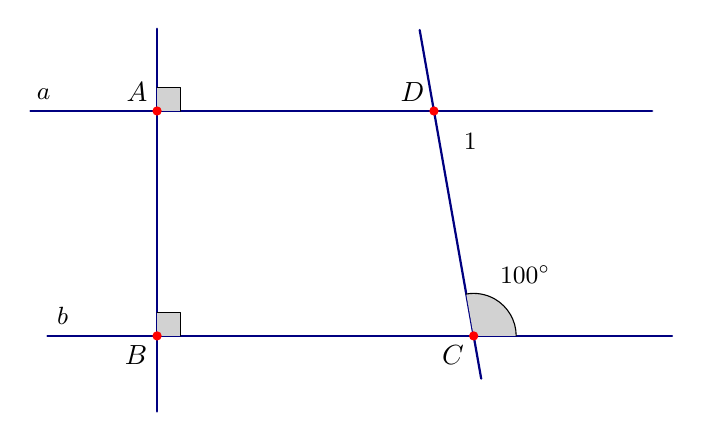
\begin{tikzpicture}[scale=1.2, line cap=round, line join=round, >=Stealth]
  % Toạ độ các điểm (1 đơn vị ≈ 1 cm, đo từ ảnh)
  \coordinate (A) at (0,0);
  \coordinate (B) at (0,-2.38);
  \coordinate (D) at (2.93,0);
  \coordinate (C) at (3.35,-2.38);   % góc C = 100° nên CD hợp với tia Cx một góc 100°

  \def\lc{blue!50!black}

  % Đường thẳng a, b
  \draw[\lc, thick] (-1.34,0) -- (5.24,0);
  \draw[\lc, thick] (-1.16,-2.38) -- (5.45,-2.38);

  % Đường thẳng AB
  \draw[\lc, thick] (0,0.87) -- (0,-3.18);

  % Cát tuyến CD (kéo dài hai đầu)
  \draw[\lc, thick] ($(D)!-0.36!(C)$) -- ($(C)!-0.19!(D)$);

  % Ký hiệu góc vuông tại A và B (cạnh 0.25 cm, nằm góc phần tư trên bên phải)
  \fill[gray!35] (0,0) rectangle (0.25,0.25);
  \draw[thin] (0.25,0) -- (0.25,0.25) -- (0,0.25);
  \fill[gray!35] (0,-2.38) rectangle (0.25,-2.13);
  \draw[thin] (0.25,-2.38) -- (0.25,-2.13) -- (0,-2.13);

  % Cung góc C = 100°
  \fill[gray!35] (C) -- ++(0:0.45) arc (0:100:0.45) -- cycle;
  \draw[thin] (C) ++(0:0.45) arc (0:100:0.45);
  \node[font=\small] at ($(C)+(50:0.85)$) {$100^\circ$};

  % Nhãn góc D_1 (nằm dưới a, bên phải CD)
  \node[font=\small] at ($(D)+(-40:0.5)$) {$1$};

  % Các điểm
  \foreach \P in {A,B,C,D}{\fill[red] (\P) circle (1.4pt);}

  % Nhãn đỉnh
  \node[above left]  at (A) {$A$};
  \node[above left]  at (D) {$D$};
  \node[below left]  at (B) {$B$};
  \node[below left]  at (C) {$C$};

  % Nhãn đường thẳng
  \node[above, font=\small] at (-1.2,0.02) {$a$};
  \node[above, font=\small] at (-1.0,-2.36) {$b$};
\end{tikzpicture}
\end{center}

\end{document}
